% jupiter-data-refinement-illustration.tex

\documentclass[tikz]{standalone}
% jupiter-illustration-preamble.tex

\usepackage{tikz}
\usetikzlibrary{shapes, positioning, arrows.meta, calc, backgrounds, fit}

\def\hdist{1.8}
\def\vdist{2.0}
\tikzset{node distance = \vdist and \hdist}

\tikzset{every lower node part/.style = {red}}
\newcommand{\statesplit}[4]{% #1: state upper label; #2: state lower label; #3: position; #4: name
  \node (#4) [circle split, draw, minimum size = 6mm, text width = 10mm, align = center, #3, font = \Large]
  {
    $#1$
    \nodepart{lower}
    $#2$
  };
}

\newcommand{\rectsplit}[2]{% #1: state upper label; #2: state lower label
  \node [draw, rectangle split, rectangle split parts = 2, 
    align = center, font = \Large]
  {
    #1
    \nodepart{two}
    \textcolor{red}{#2}
  };
}

\newcommand{\transition}[4][]{% #2: start state; #3: end state; #4: transition label; #1: transition label position (optional)
  \draw[>=Stealth, ->] (#2) to node (#2to#3) [rectangle, draw, above = 2pt, sloped, #1, font = \small] {$#4$} (#3);
}

\newcommand{\set}[1]{\{#1\}}
\newcommand{\ins}[2]{\textsc{Ins}(#1,#2)}
\newcommand{\del}[2]{\textsc{Del}(#2)}
% \newcommand{\del}[2]{\textsc{Del}(#1,#2)}


\usetikzlibrary{arrows.meta}
\usetikzlibrary{chains}

\begin{document}
\begin{tikzpicture}[bg/.style = {rectangle, draw, very thick}, node distance = 0.0cm,
    start chain = going right,
    refine/.style = {>=Stealth, ->, very thick, #1}]
  % absjupiter-c3-4
  \node (absj) [on chain, label = {[font = \Huge] above : \textsl{AbsJupiter}}] 
    {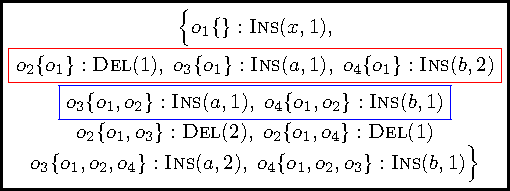
\includegraphics[scale = 1.50]{absjupiter-c3-set}};
  % cjupiter-c3-4
  \node (cj) [on chain, label = {[font = \Huge] above : \textsl{CJupiter}}] 
    {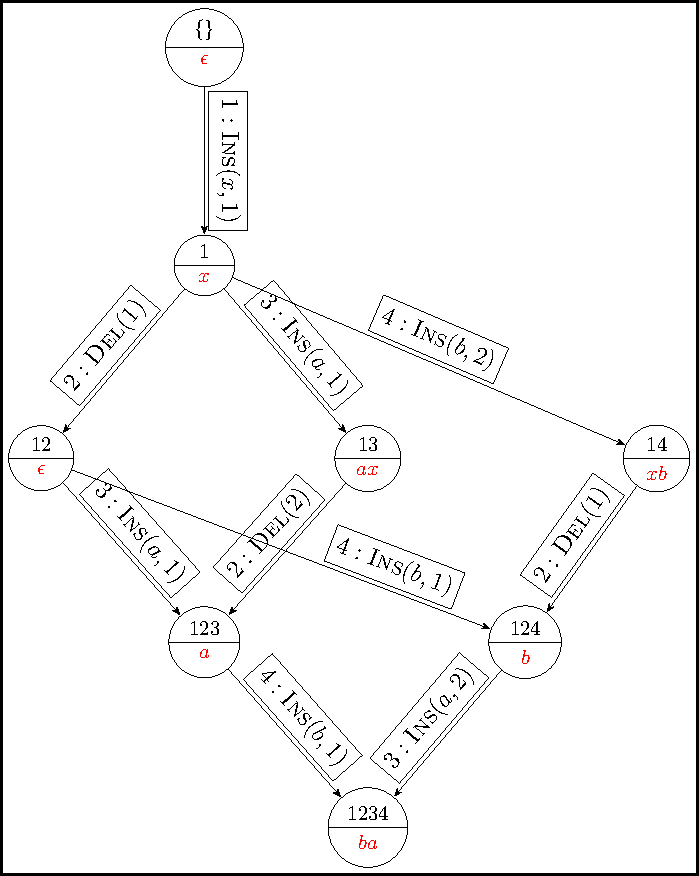
\includegraphics[scale = 1.00]{cjupiter-c3-nary-digraph}};
  % xjupiter-c3-4
  \node (xj) [on chain, label = {[font = \Huge] above : \textsl{XJupiter}}]
    {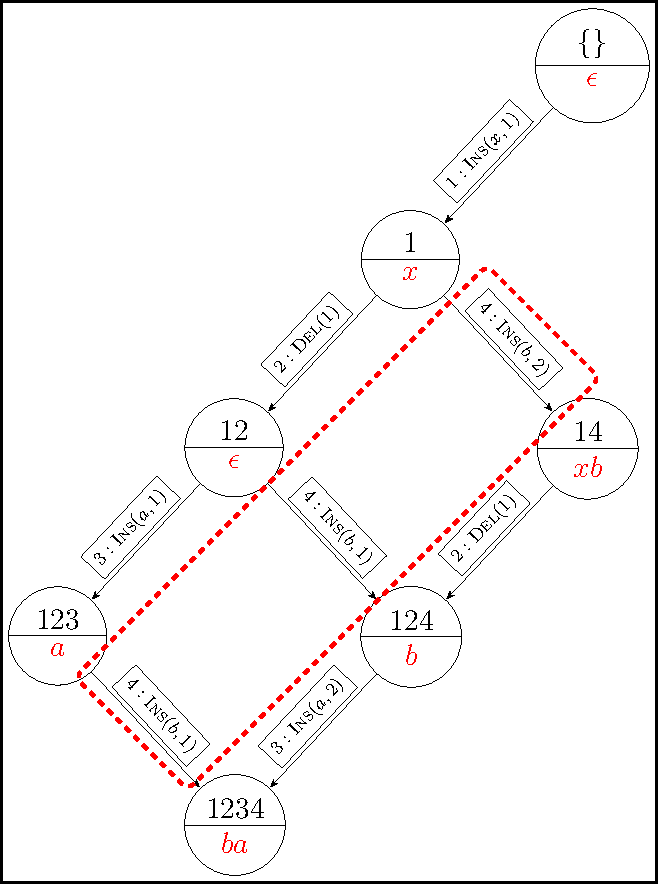
\includegraphics[scale = 1.00]{xjupiter-c3-2d-digraph}};
  % ajupiter-c3-4
  \node (aj) [on chain, label = {[font = \Huge] above : \textsl{AJupiter}}] 
    {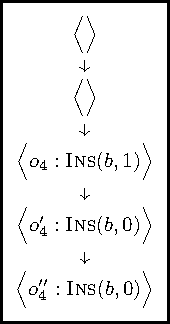
\includegraphics[scale = 1.50]{ajupiter-c3-buffer}};

  \draw [refine = {bend right = 20}] (absj.south) to node [font = \Huge, align = center] 
    {organized into $n$-ary digraph; \\ grouping $Cop$s with the same context}
    (cj.south);

  \draw [refine = {bend left = 10}] (cj.north) to node [below = 10pt, font = \Huge, align = center] 
    {optimization at the client side; \\ eliminating redundant $OT$s \\ already performed at the server}
    (xj.north);

  \draw [refine = {bend right = 20}] (xj.south) to node [font = \Huge, align = center] 
    {keep local dimension at clients; \\ keep remote dimension at the sever}
    (aj.south);
\end{tikzpicture}
\end{document}
